\documentclass{article}
\usepackage{amsmath}
\usepackage{amsfonts} 
\usepackage{graphicx}
\usepackage{biblatex} 
\usepackage{authblk}
\usepackage{mathtools}
\usepackage{xurl} %see https://tex.stackexchange.com/questions/23394/url-linebreak-in-footnote for why we use xurl to get line breaks instead of regular url
\usepackage[hidelinks]{hyperref}
\usepackage{listings}
\usepackage{cancel}
\usepackage{enumitem}
\usepackage[bb=boondox]{mathalfa}
\addbibresource{sample-base.bib}
\DeclareMathOperator*{\argmax}{arg\,max}
\DeclareMathOperator*{\argmin}{arg\,min}
\usepackage{fancyhdr}
\usepackage{textcomp}

\setlist[description]{leftmargin=2cm,labelindent=1cm}

\lstdefinestyle{mystyle}{
    % backgroundcolor=\color{backcolour},   
    % commentstyle=\color{codegreen},
    % keywordstyle=\color{magenta},
    % numberstyle=\tiny\color{codegray},
    % stringstyle=\color{codepurple},
    % basicstyle=\ttfamily\footnotesize,
    % breakatwhitespace=false,         
    % breaklines=true,                 
    captionpos=b,                    
    keepspaces=true,                 
    % numbers=left,                    
    % numbersep=5pt,                  
    % showspaces=false,                
    % showstringspaces=false,
    % showtabs=false,                  
    tabsize=2,
    frame=single,
}
\lstset{style=mystyle}

\title{The Koyote Science, LLC, Approach to Personalization and Recommender Systems}
\author[1]{Douglas Mason}
\affil[1]{\href{http://www.koyotescience.com}{Koyote Science, LLC}}
\date{February 2022}

\begin{document}

\maketitle

\tableofcontents

\pagestyle{fancy}
% \fancyhf{}
\cfoot{\\
\\
\includegraphics[scale=0.15,valign=c]{koyote_science_logo.png}
}
\lhead{Page \thepage}
\rhead{Section \thesection}

\section{Introduction}

Personalization and recommender systems present unique challenges that can be addressed with intelligent bandit design. These algorithms require less feature-engineering, and use embeddings to represents users, queries, and items, making them the go-to for products with a history of interactions to build upon. When working with new users or when substantial historical data has not been recorded, bandits can help collect this data efficiently. Moreover, while recommender systems have evolved to enormously complex extremes to accommodate signals as quickly as possible, bandits paired with recommender systems can capture user intent in the moment with little additional effort, providing a tremendous improvement over traditional approaches. This document outlines the recommender system problem, how bandits have been used to address issues in the past, and how we would do it differently.

\section{History and background}

Any developed technology company will have a well-tuned, efficient global model covering all of their customers. Such systems derive largely from \textbf{collaborative filtering}\cite{CF_survey1, CF_survey2, CF_survey3}, which boils down to singular value decomposition on the user-item matrix whose rows identify a user, whose columns identify an item, and whose entries identify interactions between the given user and item.

Side information for the users, such as demographics, as well as the items, such as genre or format, can be used in a separate recommendation method called \textbf{content-based filtering}, by which a traditional supervised learning model is trained on the user and item features, and generally include the interactions between those features. A popular elaboration includes adding contextual features to the model, such as time-of-day, or day-of-week, which opens up the possibility of hierarchical models, whereby we learn global trends as well as user-specific preferences. 

Content-based filtering is great for cold-start problems where these features are available but not prior interactions for the user, however it generally underperforms collaborative filtering once interactions have been recorded. Moreover, performance can suffer in large part because identifying meaningful features, building the appropriate data pipeline, and quality assurance are all non-trivial compared to accumulating the user-item matrix. Content-based filtering benefits from operating on traditional supervised learning methods, and can be easily integrated with any bandit or reinforcement-learning system accordingly.

Combining collaborative filtering and content-based filtering, we arrive at \textbf{hybrid recommendation models}\cite{hybrid_recommender, hybrid_recommender2}. Popular techniques in this domain include factorization machines\cite{factorization_machines, deep_factorization_machines}, which learn additional embeddings for side information features and add these to the model. A popular implementation of this style of recommender is LightFM\cite{lightFM, xLightFM} available in Python, although custom implementations can be built for businesses with the resources to do so. 

Collaborative, content-based, and hybrid filtering are all mature methods that can be used not only to recommend items like movies, songs, and books, but also how those items are displayed, such as which rows of recommended items are presented, like "Previously watched" and "Great horror classics". This can be accomplished by encoding these display elements in a separate user-item matrix or content-based filtering model and finding clever ways to use this signal. For example, the reader can see the Netflix blog entry\footnote{Source: \url{https://netflixtechblog.com/learning-a-personalized-homepage-aa8ec670359a}} which covers the topic on a very high level, mostly focusing on heuristic methods on top of the underlying signal to encourage diversity or account for causal inference.

\section{Mathematical formulation}

Using \textbf{deep learning}, that is, a neural network function approximator guided by a stochastic gradient descent style optimizer, an alternate view of factorization machines sees each user and item being converted in an \textit{embedding} or \textit{representation}, with their interactions modeled by the dot product between those embeddings. This allows us to construct extremely expressive hybrid recommender systems as a variation on linear regression with quadratic feature interactions, using the dot products between the embeddings to dramatically reduce the number of parameters that need to be learned\footnote{See \url{https://towardsdatascience.com/factorization-machines-for-item-recommendation-with-implicit-feedback-data-5655a7c749db}}. While complex deep neural networks can be used, a single-layer network equivalent to a linear regression has the benefit of being a convex optimization problem that is far more stable to solve.

We can write out our function approximator as

\begin{equation}
    f(\mathbf{x},\boldsymbol{\theta},\boldsymbol{\phi}) = \theta_0 + \sum_{p=1}^{P}\theta_p x_p + \sum_{p=1}^{P-1}\sum_{q=p+1}^{P}\boldsymbol{\phi}_p^\top \boldsymbol{\phi}_q x_p x_q
\end{equation}where 
\begin{itemize}
\item $\mathbf{x}$ is a one-hot encoding of the users and items concatenated with (possibly float-valued) contextual features like time-of-day for a given interaction,
\item  $\boldsymbol{\theta}$ is the set of (scalar) weights for each feature in $\mathbf{x}$, sometimes referred to as the user and item biases, but it also includes weights for contextual features
\item $\boldsymbol{\phi}$ is the $P\times M$ matrix of representations for each user and item as well as contextual features we would like represented this way, where $M$ is the number of embedding dimensions, although this number can depend on the user, item, or contextual feature rather than being static
\end{itemize}
Note that we don't one-hot encode the users or items explicitly but rather look them up in a dictionary defined by the model, however, the formalism is easier to write out this way. 

The model parameters $\boldsymbol{\theta}$ and $\boldsymbol{\phi}$ are optimized to minimize the standard squared-error loss\cite{CF_neural, CF_neural2},
\begin{equation}
    L(\mathbf{X},\boldsymbol{\theta},\boldsymbol{\phi}) = \frac{1}{N}\sum_{i=1}^{N}(\sigma(f(\mathbf{X}_i,\boldsymbol{\theta},\boldsymbol{\phi})) - y)^2 + \lambda \left(||\boldsymbol{\theta}||_2 +  ||\boldsymbol{\phi}||_2\right)
\end{equation}where 
\begin{itemize}
\item $N$ is the number of samples in $\mathbf{X}$
\item $\sigma$ is a link function that is the identity for a linear regression and the sigmoid function for binary outputs
\item $y$ is the measure of interest (item rankings, engagement, etc.)
\item $\lambda$ is the L2-norm regularization constant
\end{itemize}

\begin{figure}[h]
\begin{center}
  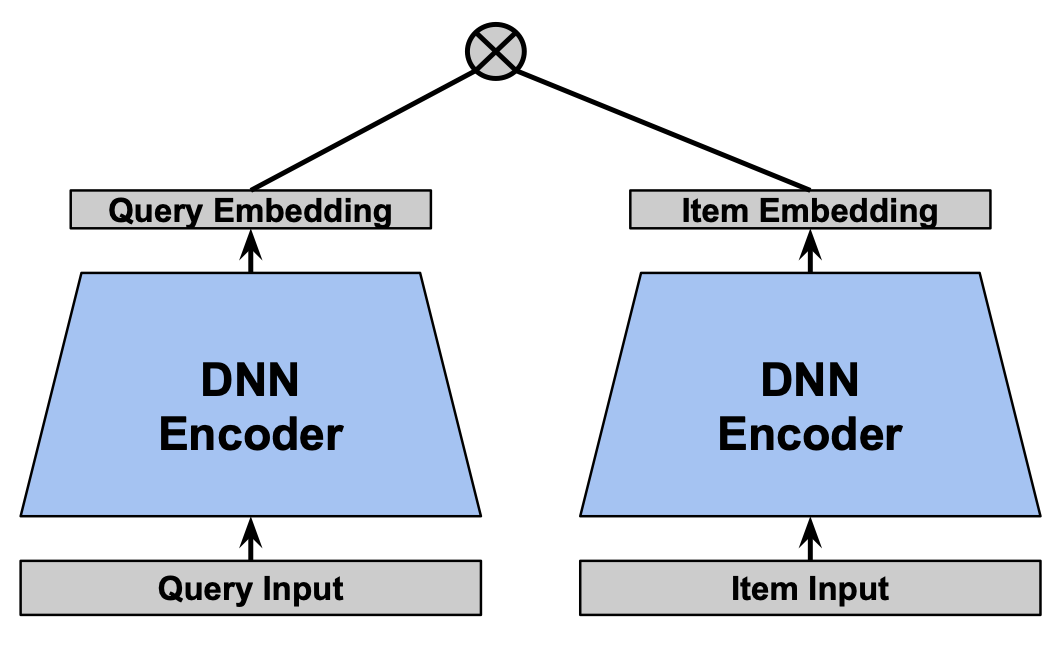
\includegraphics[width=0.75\linewidth]{two_tower.png}
  \end{center}
  \caption{The user (query) and item features can be fed into a two-tower deep neural network to learn embeddings and interaction features among each type of feature (user and item) separately. The dot product is then used to model interactions between the user and the item, and the learned embeddings can be used in any k-nearest neighbors retrieval system to find similar users or items. This flexible design allows for a variety of side-chain information, such as time-of-day, to be used in either the user tower, item tower, or both. Source: \url{https://research.google/pubs/pub50257/}}
  \label{fig:two_tower}
\end{figure}

\begin{figure}[h]
\begin{center}
  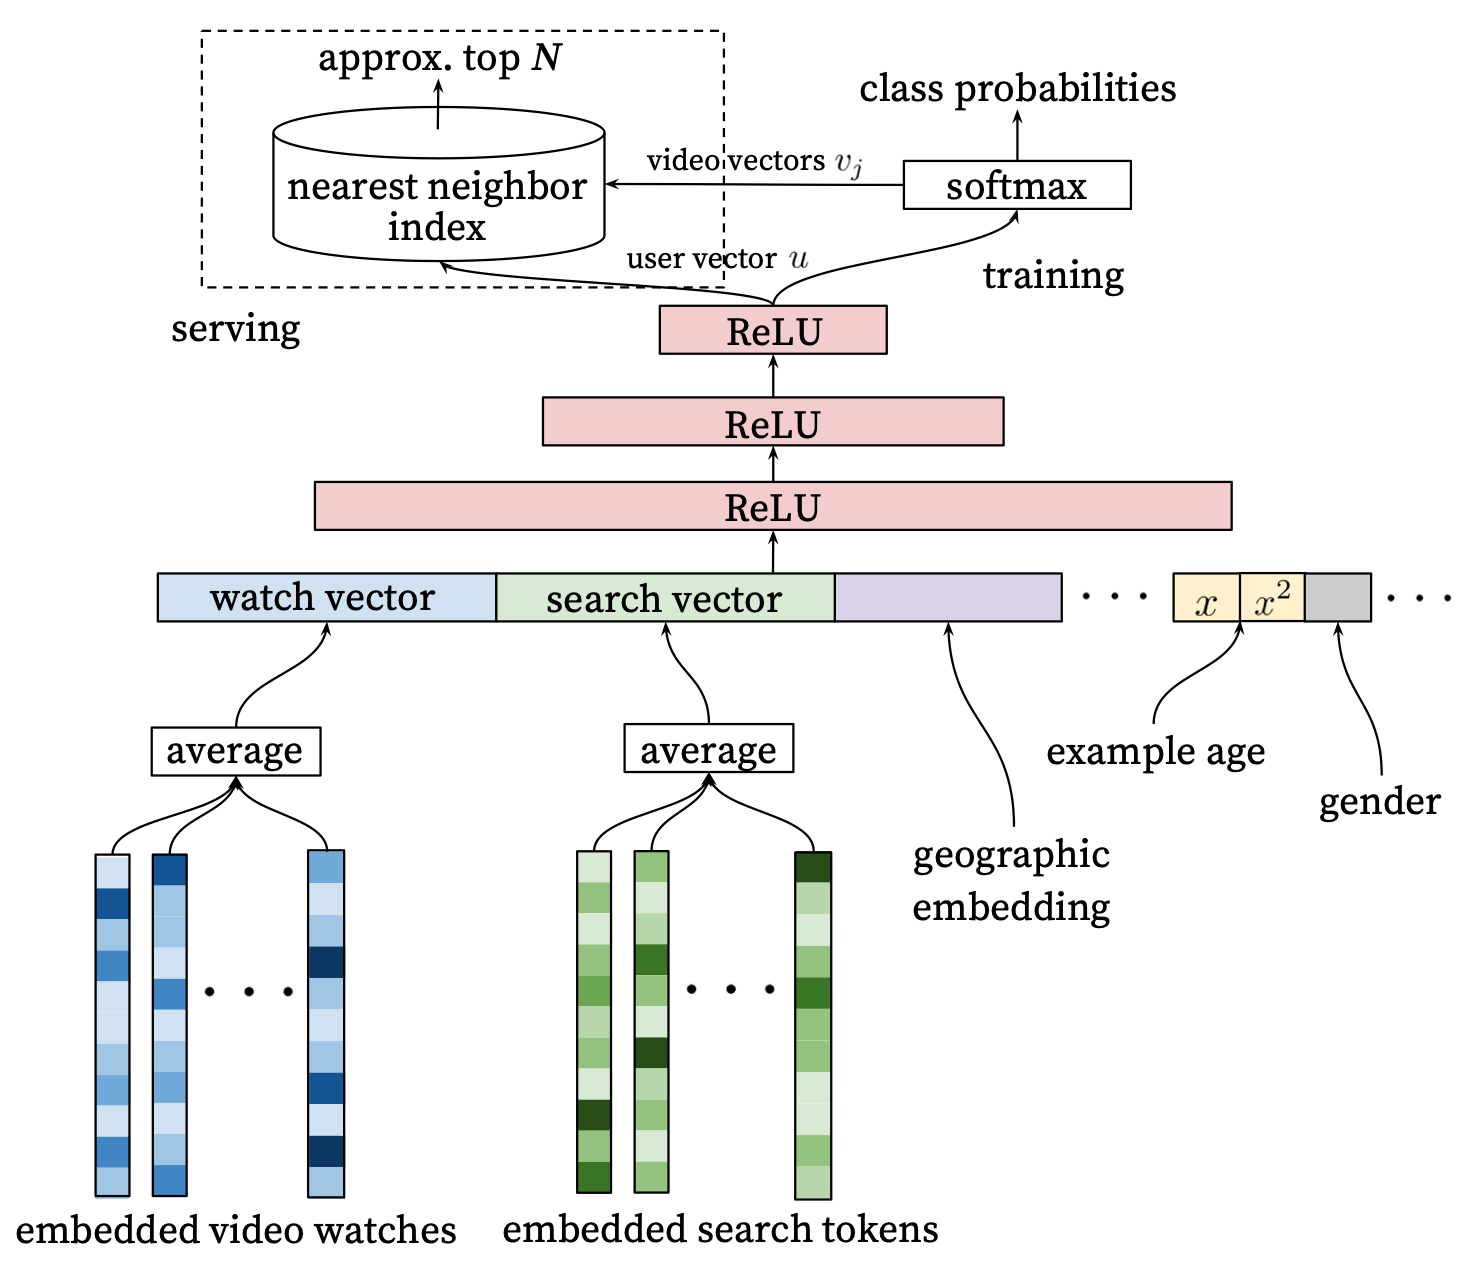
\includegraphics[width=0.75\linewidth]{youtube_figure.png}
  \end{center}
  \caption{The YouTube implementation encodes an enormous amount of side-chain information. Source: \url{https://research.google/pubs/pub45530/}}
  \label{fig:you_tube}
\end{figure}

Further elaborations include triplet losses for learning relative rankings rather than explicit predictions of $y$\cite{learning_to_rank_recsys} which is implemented with LightFM\cite{lightFM}, and deep neural networks to learn expressive representations in well-known implementations such as YouTube's\cite{youtube_recsys} (Figure \ref{fig:you_tube}) and the "two tower DNN" design\cite{google_recsys_two_tower} (Figure \ref{fig:two_tower}). In general, the more expressive the model becomes, the easier it is to program in an auto-differentiation package like JAX compared to using pre-built APIs like Keras to allow for fine-tuned control.

\section{Implicit feedback and negative sampling}

When our goal is to predict click-through-rates rather than scalar regression (such as movie ratings), but we only record \textbf{implicit feedback} (the clicks), this can impose new challenges when the number of items is large. For a small number of items, a multi-class model can predict over all items and compute the softmax explicitly, training one interaction at a time and assuming all other items were not interacted with. For multi-label models, we can collect all interactions and non-interactions for a user and train them simultaneously. 

However, when the number of items grows, we cannot model each item in our outputs due to resource constraints and are forced to use models that accept items as input vectors rather than as the set of discrete outputs. This leaves us with a multi-class softmax model that trains one interaction at a time, or a binary classification model that only predicts for a given user and item. However, if we only train on the interactions,  we must beware of the phenomenon of "folding", by which distinct clusters of data will be incorrectly assigned similar embedding values\cite{folding_without_negative_sampling_recsys}. To address this issue, \textbf{negative sampling} is employed by which we sample the non-interactions rather than use all of them. 

The negative samples can be trained explicitly for binary classification models, at which point the problem is identical to managing class imbalance, i.e., when the distribution of your training data differs from the data you infer on. Unfortunately, this approach introduces new hyperparmaters governing how we obtain the negative samples and in what proportion to include them, which are then tuned to optimize some classification goal. In our case, our goal is some metric of the recommender system, such as top-k ranking. Incidentally, these considerations amount to the importance sampling ratio used in off-policy evaluation in reinforcement learning, since we are attempting to bridge the differences between the the training data distribution the model is trained on and the inference data distribution the model will be applied on. Notably, when we only record data for one class (the interactions), we have no way to determine the importance sampling ratios a-priori, which is why we are left hyperparameters to tune.

For multi-class models, while negative samples can be included in the training data as in binary classification, they can also just be included in the normalization denominator, i.e., the partition function, in the per-sample likelihood \begin{equation}\mathcal{L}_\text{softmax}(\mathbf{a},\mathbf{c},\boldsymbol{\theta})=\frac{\exp(f(\mathbf{a},\mathbf{c},\boldsymbol{\theta}))}{\sum_{\mathbf{a}'}\exp(f(\mathbf{a}',\mathbf{c},\boldsymbol{\theta}))}
\end{equation}. The loss function \begin{equation}L(\boldsymbol{\theta})=-\frac{1}{N}\sum_{\mathbf{a},\mathbf{c}}\log\mathcal{L}_\text{softmax}(\mathbf{a},\mathbf{c},\boldsymbol{\theta})\end{equation}then averages over all actions (items) and contexts (users) in our dataset of size $N$. We don't need to explicitly train the negative samples to shift their embeddings because the gradients of the loss function related to the softmax denominator will do that for us.

Various methods are employed for selecting the negative samples, the most common and easiest-to-use being random negative sampling. However, similar to off-policy reinforcement learning, we can sample our negatives from any non-random distribution we like so long as we properly account for inverse probability weighting and importance sampling\cite{bengio_negative_sampling}. Alternatively, the user can be explicitly defined by the target-weighted sum of item embeddings that they have interacted with to avoid this issue, although this requires using sparse matrix libraries and limits the number of items that can be modeled.

Negative sampling is necessary for models where we we apply a softmax to our prediction probabilities, that is, we treat each interaction as a win against a pool of other candidates, forcing the model to rank the likelihood of the current interaction against the non-interactions. However, instead of treating this as a multi-class single-label classification problem, we can also train just to predict the interaction probability between a given user and item without the softmax function forcing a ranking among items in the model. This turns our problem into a single-value binary classification or regression problem. Once a substantial amount of interaction data has come in, the softmax approach will outperform the alternative formulation for the same reason that multi-task models learn better embeddings and improve model performance in general, and similarly, a multi-class \textit{multi-label} model using a final sigmoid activation layer over all items will perform in between. But the greater performance comes at a cost: handling missing information or heterogenous data becomes substantially more difficult since all items have to be ranked concurrently against each other. For this reason, cold-start problems often ignore the softmax function and rely on a more traditional bandit formulation.

Note that when the number of items becomes large, performing predictions for ranking becomes a substantial computational overhead. To address this, nearest-neighbor algorithms\cite{nearest_neighbors} like K-D tree and ball tree can be used to reduce the search time by searching for item embeddings that are closest to the query embedding since these will have the largest dot-products. Note that this algorithm requires the two-tower design depicted in Figure \ref{fig:two_tower}, to measure the distances between the final query and item embeddings, as well as direct access to the final embedding layers rather than building off of the model predictions, which can make the engineering a bit harder.

\section{Reinforcement learning for recommender systems}

\textbf{Reinforcement learning} has been extensively explored in the literature as a way of improving recommender systems\cite{rl_recsy, rl_recsys2, rl_recsys3}. First, we consider how it would be added to either of the above methods individually. For collaborative filtering alone, the predominant approach is to use a Bayesian implementation of matrix factorization called \textit{probabilistic matrix factorization}\cite{PMF_probabilistic_matrix_factorization,BPMF_bayesian_probabilistic_matrix_factorization} to create \textit{interactive collaborative filtering}\cite{interactive_CF,interactive_CF2,interactive_CF3} implementations which balance exploration and exploitation in data collection for the collaborative filtering signal. It remains unclear if similar approaches can be used for factorization machines. Meanwhile, content-based filtering extends to reinforcement learning trivially. 

With the deep learning formulation, it is possible to combine all three approaches satisfyingly into one formalism since it treats collaborative filtering like a content-based filtering problem. The question remains how to capture prediction uncertainty to drive RL policies and make the exploration-exploitation trade-off possible, which is what probabilistic matrix factorization solved for the classical model. You can either employ an epsilon-greedy or softmax policy based on static predictions (poor performance), or use bootstrapped ensembles for Thompson sampling\cite{randomized_prior_functions, bootstrap_DQN, thompson_sampling} which incurs greater training costs but zero latency issues for the customer. This is our preferred method because it has been shown to outperform others in many contexts\cite{thompson_sampling1, thompson_sampling2, thompson_sampling3}. Other proposals, such as MC-dropout\cite{monte_carlo_dropout} and Bayes-by-backprop\cite{bayes_by_backprop}, have not yet been proven effective or accurate\cite{risk_versus_uncertainty}

\section{How we would do it differently}

While reinforcement learning has been explored to optimize these signals as we've discussed, such efforts ignore the major benefit of the technology: enhanced and responsive interactions. For example, a feature-rich recommender system with tons of data like YouTube's can tell us your propensity to watch horror movies on a Friday night, and can even tell us when users are globally excited for the genre because Halloween is fast-approaching. By adding recent historical features, such as representations of the most-recently interacted items, advanced models can also capture sequential tendencies, such as the propensity to watch the second episode of a show that a user just started. 

However, even with enormous resources and instantaneous updates, \textbf{traditional recommenderg systems are based on static historical signals and cannot tell us about the customer in the moment.} In other words, such models can deduce your likelihood for wanting to see horror on this Friday night, but they cannot capture that intention directly, and therefore miss out on the most-important signal. Heuristic add-ons can replicate some of the desired responsiveness, but they are prone to errors in edge cases, require expensive A/B testing, and are designed by humans rather than built on sound foundational principles. In other words: we can certainly do better, and the lessons learned with bandits and reinforcement learning are the key to getting there.

The key concept here is that \textbf{any real-time signal we obtain must be extremely simple}. Recommender systems excel with enormous amounts of data, but any model that bootstraps off of their predictions and responds to users in the moment can only capture a few more nuances. We assume for the moment that we are supplied with a recommender system that provides us predictions based on historical data of user-item engagement. In the traditional linear bandit setup, we define a linear regression function approximator as
\begin{equation}
    f(\mathbf{a},\mathbf{c},\boldsymbol{\theta}) = \theta_0 + \sum_{i=1}^{N_a}\theta_i a_i+\sum_{i=1}^{N_c}\theta_{i+N_a}c_i+\sum_{i=1}^{N_a}\sum_{j=1}^{N_c}\theta_{i+jN_a+N_a+N_c} a_i c_j
\end{equation}where $\mathbf{a}$ is the $N_a$-length action feature vector, $\mathbf{c}$ is the $N_c$-length context feature vector, and $\boldsymbol{\theta}$ is the model parameters. As we can see, this model has $1+N_a+N_c+N_a\times N_c$ parameters, which is substantial! How can we reduce this number?

We instead define our features as follows. We make one model for each user and session so that the context feature vector is null.  For each item (the action) we encode the recommender system prediction between the user and item as well as any gestalt features we hope to capture about the item. We write this \textbf{simplified model} as 

\begin{equation}
    f(\mathbf{a},\boldsymbol{\theta}) = a_r+\sum_{i=1}^{N_a}\theta_i a_i
\end{equation}where we have removed the bias term $\theta_0$ since it doesn't affect rankings and replaced it with the recommender prediction $a_r$. How simple! So how would this work in practice?

Imagine that you want to capture whether a user is interested, right now, in horror. We use the simplified model in a bandit setup. We start with a prior on the parameters so that we don't begin with pure exploration set to $\boldsymbol{\theta}=\mathbf{0}$, with a prior noise parameter $\sigma_p$ tuned to how much we want to explore to begin with. As the system learns, it will discover how much it should weight its contribution against the recommender system. If $\theta_1$ is a Boolean capturing whether the item falls into horror, this model weight will capture how much we should up-recommend horror items. As we add more features to the model, we may need to tighten the prior noise parameter accordingly to capture the same level of exploitation, so this method still leaves over a hyperparameter to hand-tune, $\sigma_p$. Other models can be considered, for example, the multiplicative model
\begin{equation}
    f(\mathbf{a},\boldsymbol{\theta}) =  a_1  \sum_{i=1}^{N_a}\theta_i a_i
\end{equation}where the prior recommendation is multiplied through the parameters and features to give a desired outcome.

\section{Building probabilistic logic out of bandit components for expressive and responsive recommendation products}

Any recommender system is really a bandit or reinforcement learning algorithm in disguise, with the main difference being that collaborative filtering uses embeddings and dot products in the function approximator, while the bandit and RL literature focuses on more traditional formulations. Generally, practitioners don't concern themselves with the data collection feedback loop in a recommender system because it is assumed that there is a lot of historical data that needs to be batch-processed, and therefore the uncertainties of the predictions are assumed to be very small and irrelevant to the data collection process. However, for small-data domains like products that are bootstrapping themselves from their customers, and any cold-start or low-data user or item, this is certainly not the case (pun absolutely intended)!

There are two primary methods by which bandits and reinforcement learning components can be linked. The first, as discussed in the previous section, is to use the prediction of one bandit as a feature in another. We can further elaborate on uncertainty propagation by using not the mean prediction as our feature but a sample from the bandit's prediction distribution. Moreover, we can use predictions from multiple bandits and bandits trained on multiple rewards as input to another bandit. (Note that even though only on reward drives the policy for a given bandit, we can still train against many targets, the difference only appearing in how off-policy corrections and importance sampling are executed.) This can help ensure that we do not over-exploit too early, and is a method borrowed from the reinforcement learning literature (see, for example, randomized least squares value iteration\cite{RLSVI}).

The second way to link bandits is to use one bandit to pre-select the pool of choices for another. In this case, it is important to pass to the bandit consuming the pool the likelihood of including of including each element in the pool.  An isolated bandit will be able to compute its own likelihood for pool inclusion depending on its acquisition function, and use the inverse of this value to weight the data in the model during the training process. In the case of only one item in the pool, such as presenting a single option to the user and seeing if they engage it, this amounts to traditional inverse probability weighting as discussed in \cite{Mason_Real-World_Reinforcement_Learning_2021} and \cite{sutton_barto_rl}, a technique that is critical to off-policy learning and causal inference, and is a simplification of more-sophisticated (and difficult-to-implement) hierarchical approaches like position-based models\cite{zappella_position_based}.

What these two links between bandits achieve for us is that they enable us to build sophisticated, hierarchical systems where each component only has to excel at its prescribed task. This means that any AutoML system used to monitor and launch a bandit service can be used in a modular fashion, each module perfecting its own selection process. This is a far more-tractable solution than traditional hierarchical Bayesian modeling which require unreliable techniques like Markov-chain Monte Carlo, variational inference, or other sampling methods developed in the field, and which require experienced practitioners and experimental software to execute such as \href{http://www.pyro.ai}{Pyro},  \href{https://docs.pymc.io/en/v3/}{PyMC3}, or \href{https://mc-stan.org}{Stan}. These limitations have restricted such approaches to the domain of one-off research studies, but the system described here is straightforward to productionize and to train engineering teams to monitor and ensure quality control. In fact, in our experience motivating engineers on this field is easy because they know they are building powerful skills for the future.

\section{Pool selection, fantasies, and enforcing diversity}

The majority of reinforcement learning literature is concerned with choosing a single optimal action given a context based on what has been learned from previous training episodes. However, recommendation systems often are tasked with choosing pools of mutually-exclusive recommendations rather than single items, generally ranked by a single score, and filtered by a query criterion. In certain two-tower and other deep-learning architectures, the query is included in the ranking itself so that all items are considered. When a user selects an item from this pool, we use the inverse policy probability of choosing that item to weight the selection's data in training our model. This means that an element with a low likelihood of being chosen will have a bigger impact if it is.

However, obtaining the correct policy probabilities in these scenarios is non-trivial, and has been extensively studied in hyperparameter optimization problems\cite{parallel_hyperparameter_tuning,parallel_hyperparameter_tuning2}, where hyperparameter selections will often be used to train models in parallel, and we may not get results back until we've had to start training new models on new hyperaparameter selections. The approach in this field is to first make a copy of your model before you start the pool selection, and to make a model copy for each item you will select. Then, for each item, you select the previous pool items that have been previously selected, obtain a new samples from the performance prediction distributions for the model copy, and use those samples to train the associated model copy. While the selections will be the same as we build up the pool, the prediction scores will not, and this allows us to sample the distribution of possibilities similar to Thompson sampling. These selections with their predicted performances are called "fantasies" and are used to sample how uncertainty may propagate during pool selection.

In reinforcement learning problems with a fixed and small number of items or actions, each one is equally available or filtered out completely, but when the availability is limited and exhibits a continuous distribution, we must make some adjustments. In particular, we must multiply the inverse probability weight by the inverse probability of having that item available as a selection. This arises because if an item was unlikely to be included in the selection, this further increases the surprise of choosing it, and averaged over many trials, we must account for it. For this situation, it is important to compute the probability of including each item in the selected pool, rather than the probability of recommending each item individually, in order to properly employ inverse probability weighting.  More-advanced approaches use a hierarchical model to model click-through rates as a function of presentation position\cite{zappella_position_based}, but this is an advanced research field that is beyond the scope of this document.

Given a sequence of items $i(s)$ selected at each step $s$, with policy probability $\pi(i(s), s)$ and availability probability $a(i(s), s)$, we compute the probability for item $i'$ at step $s'$ using the recursive equation \begin{equation}
P(i',s')=\prod_{s=1}^{s'-1} P(i(s),s)\times a(i'(s'),s')\times \pi(i'(s'),s')
\end{equation}However, this is only for the given trajectory of items $i(s)\forall s<s'$, and we must sum our probabilities over all possible trajectories. This computation is in general intractable, although we can approximate it using sampling: create $N$ different trajectories with selection sequences that are mutually exclusive of each other, and then add them up. Note that the probabilities over all items for a given step must add up to one and are constant, even though we may have different prediction score samples for a given item over different trajectories. 

For non-deterministic policies like we assume in our construction of fantasies using Thompson sampling, for each trajectory, create $M$ different probability sequences with the same selections but with different samples of the prediction distribution used to train the model copy, and average over the probability sequences for each $n\leq N$ trajectory. This approximation will converge to the true total as $N$ and $M$ grow large, although in experience only a handful of such trajectories are necessary. High-probability items will tend to dominate, and each successive trajectory contributes smaller overall probabilities since we are specifically excluding the popular choices made in previous trajectories.

It is possible some unlikely trajectory or probability sequence could swamp the probability distribution in an unexpected way, and this is why advanced Bayesian inference techniques were invented in the first place. However, they are generally never put into production because they are unstable, require hand-holding, their contributions are expensive to compute, and they are unlikely to have much impact on the final result. The bespoke algorithm MOE, which integrates over the performance probabilities of each selection\cite{scott_clark}, is another possibility, but it is unclear whether it provides a meaningful improvement given the substantial dependency it creates.

When selecting a pool of items, a common desire is to increase the diversity within it, but diversity always comes at the cost of predicted performance for the recommender system. For this reason, there is no free lunch -- we must choose what that trade-off will be, and as a result there are countless approaches to the problem, and we refer the reader to \cite{recsys_diversity_survey, netflix_recommender_system} for a detailed review.  
Our approach increases diversity in our selection pool by using Thompson sampling in our selection process and we resample the effect of each item on successive item uncertainties in the pool. While this reduces predicted performance for any given selection, it actually improves performance long term as it navigates the exploration-exploitation trade-off.

In addition, we enable a few tunable parameters for increasing the diversity: 
\begin{enumerate}
\item the fraction of selections that are truly random
\item a multiplier on the variance of our selections
\item a multiplier on the self-entropy (randomness) in our loss function
\end{enumerate}
Note that for the first tunable parameter, selections are still limited by the pool of consideration, i.e., the query filter. It is generally undesirable to introduce new tunable parameters that must be experimented on. Among the options provided here, we are least likely to recommend using the first parameter since it may have unintended consequences, while the second and third naturally converge to standard behavior when the multiplier goes to zero and one respectively. However, tunable parameters allow us to account for another type of uncertainty that Thompson sampling does not: the data could be corrupted, the measurements may be inaccurate, etc., so enhancing exploration a bit often helps accommodate these issues.

%%
%% The acknowledgments section is defined using the "acks" environment
%% (and NOT an unnumbered section). This ensures the proper
%% identification of the section in the article metadata, and the
%% consistent spelling of the heading.
%%\begin{acks}
%%To Robert, for the bagels and explaining CMYK and color spaces.
%%\end{acks}

%%
%% The next two lines define the bibliography style to be used, and
%% the bibliography file.


\printbibliography
\end{document}
